% 	TEMPLATE DE RELACIÓN DE EJERCICIOS
%
% Creador: Juamagdev

% ------------------------------------------------------------------
% ---------------------- Package imports ---------------------------
% ------------------------------------------------------------------
\documentclass[11pt, a4paper]{exam}
\usepackage[utf8]{inputenc}		% UTF-8
\usepackage[english]{babel}		% Idioma
\usepackage{graphicx}			% Para importar gráficos
\usepackage{amsthm, amsfonts, amssymb, amssymb} % Todos los paquetes AMS
\usepackage{mathtools}          % Arregla bugs de AMS
\usepackage{hyperref}			% Para \href{URL}{text}
\usepackage{enumitem}			% Para enumerar
\usepackage{color} 				% Para definir colores nuevos
\usepackage{lastpage}			% Para \pageref{LastPage}
\usepackage{booktabs}					% Tablas profesionales
\usepackage{parskip}					% Espacio de párrafos
\usepackage[sharp]{easylist}			% Para litas
\usepackage[expansion=false]{microtype} % Soluciona bugs de tipografias
\usepackage[margin=2.25cm, includehead, includefoot]{geometry}
\usepackage{cancel}
\usepackage{pgfplots}
\usepackage{listings}



% ------------------------------------------------------------------
% ---------------------- Constantes --------------------------------
% ------------------------------------------------------------------
% Las constantes mas importantes
\newcommand{\mytitle}{Ejercicio voluntario Tema 2}
\newcommand{\mysubject}{Métodos Numéricos I}
\newcommand{\mydate}{\today}
\newcommand{\myauthor}{Juan Manuel García Delgado}

% Redefinir para cada caso
\newcommand{\myrhead}{Universidad de Málaga}
\newcommand{\mypagename}{Página}
\newcommand{\mycreated}{Creado por: }
\newcommand{\mysolname}{Solución}
\renewcommand{\solutiontitle}{\noindent\textbf{\mysolname.}\hspace{0.75em}}
\pointpoints{point}{points}

\providecommand{\abs}[1]{\lvert#1\rvert}

% ------------------------------------------------------------------
% ---------------------- Ajustes -----------------------------------
% ------------------------------------------------------------------
% \shadedsolutions
\printanswers % Alternative: \noprintanswers, \printanswers
%\rhead{{\scshape {\footnotesize  \myrhead}}}
%\cfoot{\mypagename \enspace \thepage}
\definecolor{SolutionColor}{rgb}{0.8,0.9,1} % light blue

% Cabeceras y pie de página
\runningfootrule
\firstpagefootrule
\firstpagefooter{\mysubject}{}{\mypagename\ \thepage\ de \pageref*{LastPage}}
\runningfooter{\mysubject}{}{\mypagename\ \thepage\ de \pageref*{LastPage}}
\runningheader{}{}{
\includegraphics[width = 3 cm]{figs/logo.pdf}}
\firstpageheadrule
\firstpageheader{\mydate}{\mytitle}{\pageref*{LastPage} páginas en total}

% Answer command for double lines
\def\answer#1{\underline{\underline{#1}}}

% ------------------------------------------------------------------
% ---------------------- Documento ---------------------------------
% ------------------------------------------------------------------
\begin{document}
\pagestyle{headandfoot}
\noindent {\scshape \Large  \mytitle
    \ifprintanswers
        \enspace (\mysolname	 )
    \fi
} \\
\noindent {\mycreated \enspace  \myauthor} \vspace{1em}
\hrule \hrule
\vspace{5mm}

% ------------------------------------------------------------------
% ---------------------- Contenido ---------------------------------
% ------------------------------------------------------------------

\begin{questions}
    \addpoints
    \question {\bfseries Para una función dada $f: \mathbb{R} \rightarrow \mathbb{R}$, consideramos la iteración definida por}

    \begin{equation*}
        0 = f(x_k) + \frac{f(x_k) - f(x_{k-1})}{x_k - x_{k-1}}(x_{k+1} - x_k), \ \ \ \ \ \ k \leq 1
    \end{equation*}
    \textbf{con $x_0, x_1$ dados.}
    \begin{parts}
        \part Dar una interpretación geometrica del método. 
        \begin{solution}
            Primero de todo, despejamos el término $x_{k+1}$, de tal forma que nos queda: 

            \begin{equation*}
                x_{k+1} = x_k - f(x_k)\frac{x_k - x_{k-1}}{f(x_k) - f(x_{k-1})}
            \end{equation*}

            Esa expresión coincide con el \textit{Método de la Secante}. Dicho método trata de aproximar la solución de una ecuación de 
            la forma $f(x)=0$. Consiste en un algoritmo recursivo, que mientras mas iteraciones hagamos, con más precisión encontraremos un valor de la solución.

            Para entender el método, vamos a estudiar un ejemplo en concreto, como puede ser la ecuación $f(x) =0$, donde $f: \mathbb{R} \rightarrow \mathbb{R}$, con $f(x) = x + e^x$.

            Como $f(-2) = -2 - e^{-2} \approx -2.13 < 0$ y $f(2) = 2 + e > 0$, y $f$ es continua, así que por el \textit{Teorema de Bolzano} sabemos de la existencia de al menos una solucion en $(-2,2)$.
            \begin{center}
                \begin{tikzpicture}
 
                    \begin{axis}[
                        xmin = -1.5, xmax = 1.5,
                        ymin = -1.5, ymax = 4, 
                        axis x line=middle,
                        axis y line=middle]
                        
                        \addplot[
                            domain = -4:4, blue
                        ] {x + exp(x)};
                    \end{axis}
                     
                    \end{tikzpicture}
            \end{center}
            
            Para usar el método, elegimos dos puntos, en este caso $x_0 =-1$ y $x_1 = 1$. Con estos dos puntos podemos hallar su recta, que tendra de ecuación: 
            \begin{equation*}
                y - y_0 = \frac{y_0 - y_1}{x_0 - x_1}(x - x_0)
            \end{equation*}
            Entonces, como: 

            \begin{equation*}
                y_0 = f(x_0) = -1 + e^{-1}, \ \ \ \ \ \ \  y_1 = f(x_1) = 1 + e
            \end{equation*}
            Se tiene que la ecuación de la primera recta es: 
            \begin{equation*}
                y + 1 - e^{-1} = \frac{-2 + e^{-1} - e}{-2}(x+1)
            \end{equation*}

            \begin{center}
                \begin{tikzpicture}
 
                    \begin{axis}[
                        xmin = -1.5, xmax = 1.5,
                        ymin = -1.5, ymax = 4, 
                        axis x line=middle,
                        axis y line=middle]
                        \addplot[
                            domain = -4:4, red
                        ] {(-2+exp(-1) - exp(1))/(-2)*(x+1) -1 + exp(-1)};

                        \addplot[
                            domain = -4:4, blue
                        ] {x + exp(x)};
                    \end{axis}
                     
                    \end{tikzpicture}
            \end{center}

            Ahora, basta con ver que punto de la recta corta con el eje $x$ y ya tendremos el nuevo $x_2$, en este caso, $x_2 = -0,7093$. 
            Observemos que $x_2 \in (-2,2)$, luego podemos continuar con las iteraciones. 

            Ahora consideramos los puntos $(x_2, f(x_2))$ y $(x_1, f(x_1))$, y esta nueva recta (que la trazaremos de color naranja), 
            la intersecamos con el eje de ordenadas $y = 0$, y obtendremos el $x_3$, un nuevo valor más próximo a la solución que buscamos.
            
            \begin{equation*}
                y_2 = f(x_2) = -0,7093 + e^{-0,7093}, \ \ \ \ \ \ \  y_1 = f(x_1) = 1 + e
            \end{equation*}

            Luego la nueva recta es:
            \begin{equation*}
                y -1 -e = \frac{1+e+0,7093 - e^{-0,7093}}{1 + 0,7093}(x-1)
            \end{equation*}

            \begin{center}
                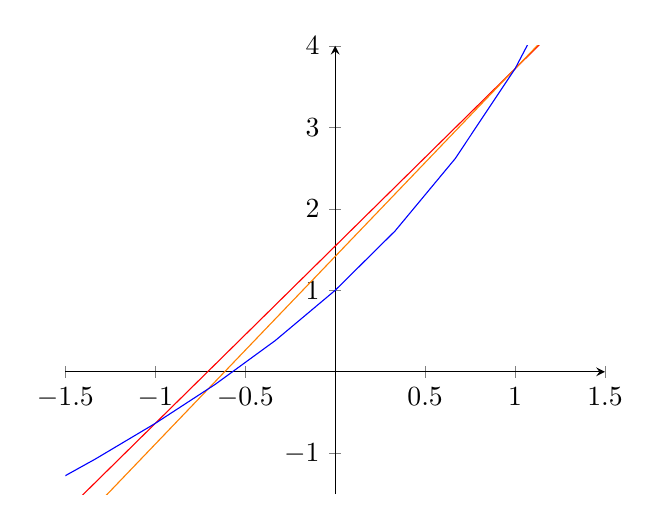
\begin{tikzpicture}
 
                    \begin{axis}[
                        xmin = -1.5, xmax = 1.5,
                        ymin = -1.5, ymax = 4, 
                        axis x line=middle,
                        axis y line=middle]
                        \addplot[
                            domain = -4:4, red
                        ] {(-2+exp(-1) - exp(1))/(-2)*(x+1) -1 + exp(-1)};

                        \addplot[
                            domain = -4:4, orange
                        ] {1 + exp(1) + 0.7093 - exp(-0.7093))/(1.7093)*(x-1) +1 + exp(1)};
                        % {(1 + exp(1) + 0,7093 - exp(-0,7093))/(1,7093)*(x-1) +1 - exp(1)
                        \addplot[
                            domain = -4:4, blue
                        ] {x + exp(x)};
                    \end{axis}
                     
                    \end{tikzpicture}
            \end{center}

            En este caso, al intersecar como se menciona anteriormente, obtenemos el nuevo $x_3$, que en este caso, $x_3 = -0,6149$.

            Ahora bastaría con repetir el proceso el número de iteraciones deseeadas hasta obtener una solución con el margen de precisión deseado. 

            En este caso, la solución es $x \approx -0.567143$. Esto se puede comprobar facilmente con un simple programa de Python como el siguiente: 


            \begin{lstlisting}[language=Python]

from numpy import *
from matplotlib.pyplot import *

import sys
sys.setrecursionlimit(100) #para evitar errores recursivos

x0, x1, cont = -1, 1, 0

def f(x):
    return x + exp(x)

def secantMethod(x0, x1, cont):
    cont += 1
    if cont > 15:
        return x1
    else:
        xs = x1 - f(x1)*(x1 - x0)/(f(x1) - f(x0))
        return secantMethod(x1, xs, cont + 1)

print(secantMethod(x0, x1, cont))
            \end{lstlisting}

        \end{solution}

        \part Si $r$ es una raíz simple de $f$, demostrar que $e_k = x_k - r$ satisface, para $x_k$ suficientemente cerca de r, que 

        \begin{equation*}
            e_{k+1} \approx \frac{f''(r)}{2f'(r)}e_ke_{k-1}
        \end{equation*}
        \begin{solution}
            Sea $r$ la raiz $f(x)=0$, y sea $x_k$ su valor aproximado usando el método de la secante tras hacer $k$ iteraciones. 

            El enunciado nos dice que se verifica para un $x_k$ lo suficientemente cerca de $r$, esto quiere decir, en un lenguaje "poco matemático" que la diferencia entre la raiz y la aproximación es mínima, o 
            lo que es lo mismo, que existe un $\epsilon > 0$ tal que: 
            \begin{equation*}
                \abs{r - x_k} \leq \epsilon
            \end{equation*}

            Se puede elegir un $k$, tal que $x_k$ y $x_{k-1}$ esten lo suficientemente cerca, o lo que es lo mismo, que para el mismo $\epsilon$ anterior, se cumpla: 

            \begin{equation*}
                \abs{r - x_k} \leq \abs{r - x_{k-1}} \leq \epsilon
            \end{equation*}

            Con esto, podemos aplicar el siguiente resultado, que usaremos para la prueba. La definición de derivada en un punto es: 
            \begin{equation*}
                f'(a) = \lim_{x \to a}\left(\frac{f(x) - f(a)}{x-a}\right)
            \end{equation*}

            Como $x_k$ es una buena aproximación a $r$, al igual que $x_{k-1}$, podemos aproximar el valor de la derivada de la siguiente forma:
            \begin{equation*}
                \frac{f(x_k) - f(x_{k-1})}{x_k - x_{k-1}} \approx f'(r)
            \end{equation*}

            Además, por el \textbf{Teorema de Taylor}, aplicado para $n =2$, tenemos que que para $x_k$ y $x_{k-1}$ lo suficientemente cerca: 

            \begin{equation*}
                f(x_k) \approx \cancel{f(r)} + \frac{f'(r)}{1!}e_n + \frac{f''(r)}{2!}e_n^2 \ \ \Rightarrow \ \ \frac{f''(r)}{2!}e_n^2 \approx f(x_k) - f'(r)e_k
            \end{equation*}

            Entonces tenemos que: 
            
            \begin{equation*}
                e_{k+1} = x_{k+1} - r = x_k - f(x_k)\frac{x_k - x_{k-1}}{f(x_k) - f(x_{k-1})} - r = 
            \end{equation*}

            \begin{equation*}
                = e_k - f(x_k)\frac{x_k - x_{k-1}}{f(x_k) - f(x_{k-1})} = \frac{e_k(f(x_k) - f(x_{k-1})) - f(x_k)(x_k-x_{k-1}))}{f(x_k) - f(x_{k-1})} = 
            \end{equation*}

            \begin{equation*}
                = \frac{x_k - x_{k-1}}{f(x_k) - f(x_{k-1})} \left(e_k\frac{f(x_k) - f(x_{k-1})}{x_k - x_{k-1}} - f(x_k) \right) = 
            \end{equation*}

            \begin{equation*}
                \approx \frac{1}{f'(r)}\left(e_kf'(r) - f(x_k)\right) = \frac{1}{f'(r)}\frac{f''(r)}{2}e_k^2 \approx \frac{f''(r)}{2f'(r)}e_ke_{k-1}
            \end{equation*}

            que es justo lo que queríamos probar. 
            
            \textit{NOTA: En las expresiones anteriores se ha usado la \textbf{aproxiomación de la derivada en un punto} y el \textbf{Teorema de Taylor}}
        \end{solution}

        \part Deducir a partir del apartado anterior que existe una constante $D>0$ tal que: 
            \begin{equation*}
                e_{k+1} \approx De_k^p, \ \ \ \ \  p = \frac{1 + \sqrt{5}}{2}
            \end{equation*}

        \begin{solution}
            Como ocurría en el caso del \textit{Método de Newton}, tomando una semilla $x_0$ lo suficientemente próxima a la raiz se obtiene la convergencia, pero 
            en la práctica, puede ocurrir que elijamos un $x_0$ por el que no obtengamos la solución, es decir, que no sea convergente la sucesion de iteraciones recursivas.

            En este caso, puede ocurrir lo mismo pero con dos valores $x_0, x_1$, es por ello que lo que nos piden es que estudiemos su ratio de convergencia. 

            Para determinar este orden de convergencia, suponemos que: 
            \begin{equation*}
                e_{n+1} \approx Ae_n^\alpha
            \end{equation*}
            donde $A$ es una constante, luego para algún $A>0$: 
            \begin{equation*}
                e_{n+1} \approx A e_n^\alpha \ \Rightarrow \ e_n \approx Ae_{n-1}^\alpha \ \Rightarrow \ e_{n-1} = (A^{-1}e_n)^{1/\alpha}
            \end{equation*}
            Por tanto, si $C = A^2$, y por la expresión del apartado b:
            \begin{equation*}
                e_{n+1} = Ae_n^\alpha = Ce_ne_{n-1} = Ce_n(A^{-1}e_n)^{1/n}
            \end{equation*}
            Luego, 
            \begin{equation*}
                Ae_n^\alpha = Ce_n(A^{-1}e_n)^{1/\alpha} \ \Rightarrow \ \frac{A^{1-1/\alpha}}{C} = e_n^{1-\alpha + 1/\alpha}
            \end{equation*}
            
            Ahora, como la primera parte es un producto de constantes, la parte de la derecha debe ser también una constante, o lo que es lo mismo, que cuando $n \rightarrow \infty$, la expresión converja. Veamos para que valores de $\alpha$ converge. 
            
            - Si $1 - \alpha + \frac{1}{\alpha} > 0$ es claro que no converge. 
            
            - Si $1 - \alpha + \frac{1}{\alpha} < 0$ es claro converge a $0$, pero esto no noss sirve. 

            Por tanto, solo nos valdrá para cuando: 
            \begin{equation*}
                1 - \alpha + \frac{1}{\alpha} = 0 \Rightarrow \alpha^2 - \alpha - 1 = 0 \Rightarrow \alpha = \frac{1 + \sqrt5}{2} 
            \end{equation*}
            que es justo lo que queríamos probar.

        \end{solution}
    \end{parts}
\end{questions}



%\hrule
%\subsection*{For retting}
%Ikke skriv noe her. \par \noindent
%\gradetable[h][questions]	
\end{document}